%% LyX 2.3.7 created this file.  For more info, see http://www.lyx.org/.
%% Do not edit unless you really know what you are doing.
\documentclass[aspectratio=169]{beamer}
\usepackage{lmodern}
\renewcommand{\sfdefault}{lmss}
\renewcommand{\ttdefault}{lmtt}
\usepackage[T1]{fontenc}
\usepackage[utf8]{inputenc}
\setlength{\parindent}{0cm}
\usepackage{amssymb}
\usepackage{graphicx}

\makeatletter
%%%%%%%%%%%%%%%%%%%%%%%%%%%%%% Textclass specific LaTeX commands.
% this default might be overridden by plain title style
\newcommand\makebeamertitle{\frame{\maketitle}}%
% (ERT) argument for the TOC
\AtBeginDocument{%
  \let\origtableofcontents=\tableofcontents
  \def\tableofcontents{\@ifnextchar[{\origtableofcontents}{\gobbletableofcontents}}
  \def\gobbletableofcontents#1{\origtableofcontents}
}

%%%%%%%%%%%%%%%%%%%%%%%%%%%%%% User specified LaTeX commands.
%\usetheme{Warsaw}
%\usetheme{Pittsburgh}
\usetheme{Oxygen}
% or ...

%\setbeamercovered{transparent}
%\setbeamertemplate{headline}{}

\setbeamercovered{dynamic}
\setbeamertemplate{navigation symbols}{}


\definecolor{blue}{RGB}{0,102,255}
\definecolor{Babyblue}{rgb}{0.54, 0.81, 0.94}
\definecolor{mainblue}{RGB}{51, 51, 178}

\usepackage{color, colortbl}
\usepackage{xcolor}
\usepackage[utf8]{inputenc}

\usepackage{movie15}
\usepackage{animate}
\usepackage{graphicx}

\usepackage{array}
\usepackage{booktabs}
\usepackage{amssymb}
\usepackage{svg}
\usepackage{media9}
\usepackage{ulem}
\usepackage{amssymb}
\usepackage{pifont}


%\renewcommand\makebeamertitle{{\logo{
\includegraphics[width=4cm]{assets/EscudoUN-2016_styledv2.png}\vspace{0.75cm}}\maketitle}}
\renewcommand\makebeamertitle{{
	\setbeamertemplate{headline}{} 
	\setbeamertemplate{footline}{} 
	\begin{frame}{} 
		\vspace{0cm}     
		\titlepage
	\end{frame}
}}


\newcommand\ungraphic{{
	\vspace{-0.5cm}
	
\includegraphics[width=0.1\textwidth]{assets/EscudoUN.png}\\
	\scriptsize{
		Universidad Nacional de Colombia\\
		Signal Processing and Recognition Group - SPRG\\
		Manizales, Colombia\\
		\today
	}
}}

\makeatother


\begin{document}
\title[Multimodal Data Exchange Systems for Enhanced Interaction and Management]{Multimodal Data Exchange System for\\Enhanced Interaction and Management}
\author{Yeison Nolberto Cardona-Álvarez}
\institute{\textbf{Advisor:} Andrés Marino Álvarez-Meza, Ph.D\\
\textbf{Co-Advisor:} César Germán Castellanos-Domínguez, Ph.D}
\titlegraphic{\ungraphic}
\date{}

\makebeamertitle

%% \AtBeginSection[]{\frame<beamer>{\frametitle{Outline}\tableofcontents[currentsection,currentsubsection]}}

\let\oldcite\cite
\renewcommand*\cite[1]{{\color {gray}\tiny{\oldcite{#1}}}}

\begin{frame}{Outline}

\tableofcontents{}
\end{frame}

\section{Motivation}
\begin{frame}{Motivation}

\framesubtitle{Data Exchange: Definition}

Data Exchange refers to the \textbf{efficient and secure} flow of
data between different platforms and procedures \cite{zhang2021fault,thakare2021secure}.

\vfill{}

\begin{figure}
\centering{}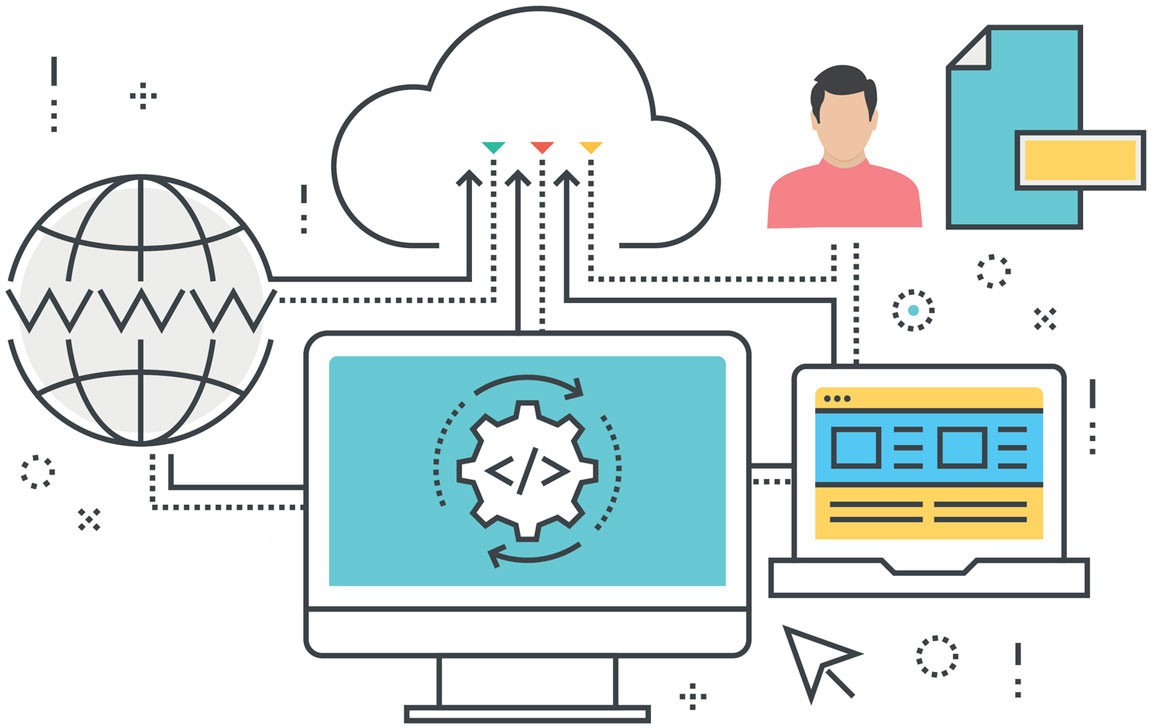
\includegraphics[width=0.3\textwidth]{images/data_exchange_1}
\end{figure}
 

\end{frame}
%
\begin{frame}{Motivation}

\framesubtitle{Data Exchange: Applications and Investments}

It requires strong security and encryption, data quality and dependability,
and industry-specific \textbf{compliance standards} \cite{attiogbe2021advances}.
\begin{columns}[t]

\column[b]{0.66\textwidth}
\begin{itemize}
\item {\scriptsize{}Business intelligence and analytics \cite{kouper2021challenges}. }{\scriptsize\par}
\item {\scriptsize{}Finance and banking \cite{Elsaify2021Data}.}{\scriptsize\par}
\item {\scriptsize{}Government and public services \cite{Ball2020Organizational}.}{\scriptsize\par}
\item {\scriptsize{}Marketing and advertising \cite{mishra2023application}.}{\scriptsize\par}
\item {\scriptsize{}Healthcare \cite{al2022application}.}{\scriptsize\par}
\item {\scriptsize{}Research and academia \cite{qiu2021comprehensive,paltun2021diverse,adiga2022enhancing}.}{\scriptsize\par}
\end{itemize}

\column[b]{0.34\textwidth}

{\scriptsize{}}{\scriptsize\par}

\begin{figure}
\centering{}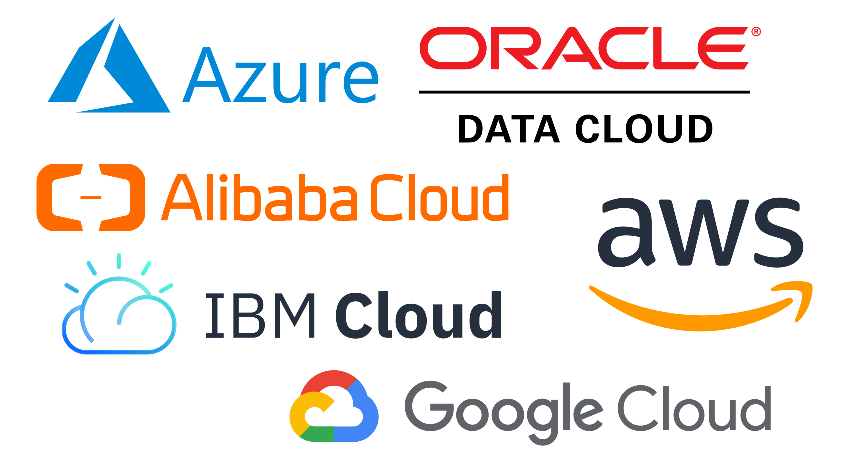
\includegraphics[width=1\columnwidth]{images/datacenters}
\end{figure}

\end{columns}

\end{frame}
%
\begin{frame}{Motivation}

\framesubtitle{The Growth of Data Centers in Colombia}

Latin America's technological revolution plays a crucial role in promoting
\textbf{regional economic growth}, closing the digital gap, creating
a foundation for improved connectivity, innovation, and robust digital
infrastructure \cite{KearneyGlobalServices2023}.
\begin{columns}[t]

\column[b]{0.6\textwidth }
\begin{itemize}
\item {\scriptsize{}Fourth largest data center market in Latin America.
}{\scriptsize\par}
\item {\scriptsize{}Significant investments in infrastructure. }{\scriptsize\par}
\item {\scriptsize{}Attractive for international investments. }{\scriptsize\par}
\item {\scriptsize{}Strategic location advantage. }{\scriptsize\par}
\end{itemize}

\column[b]{0.4\textwidth }

\begin{figure}
\centering{}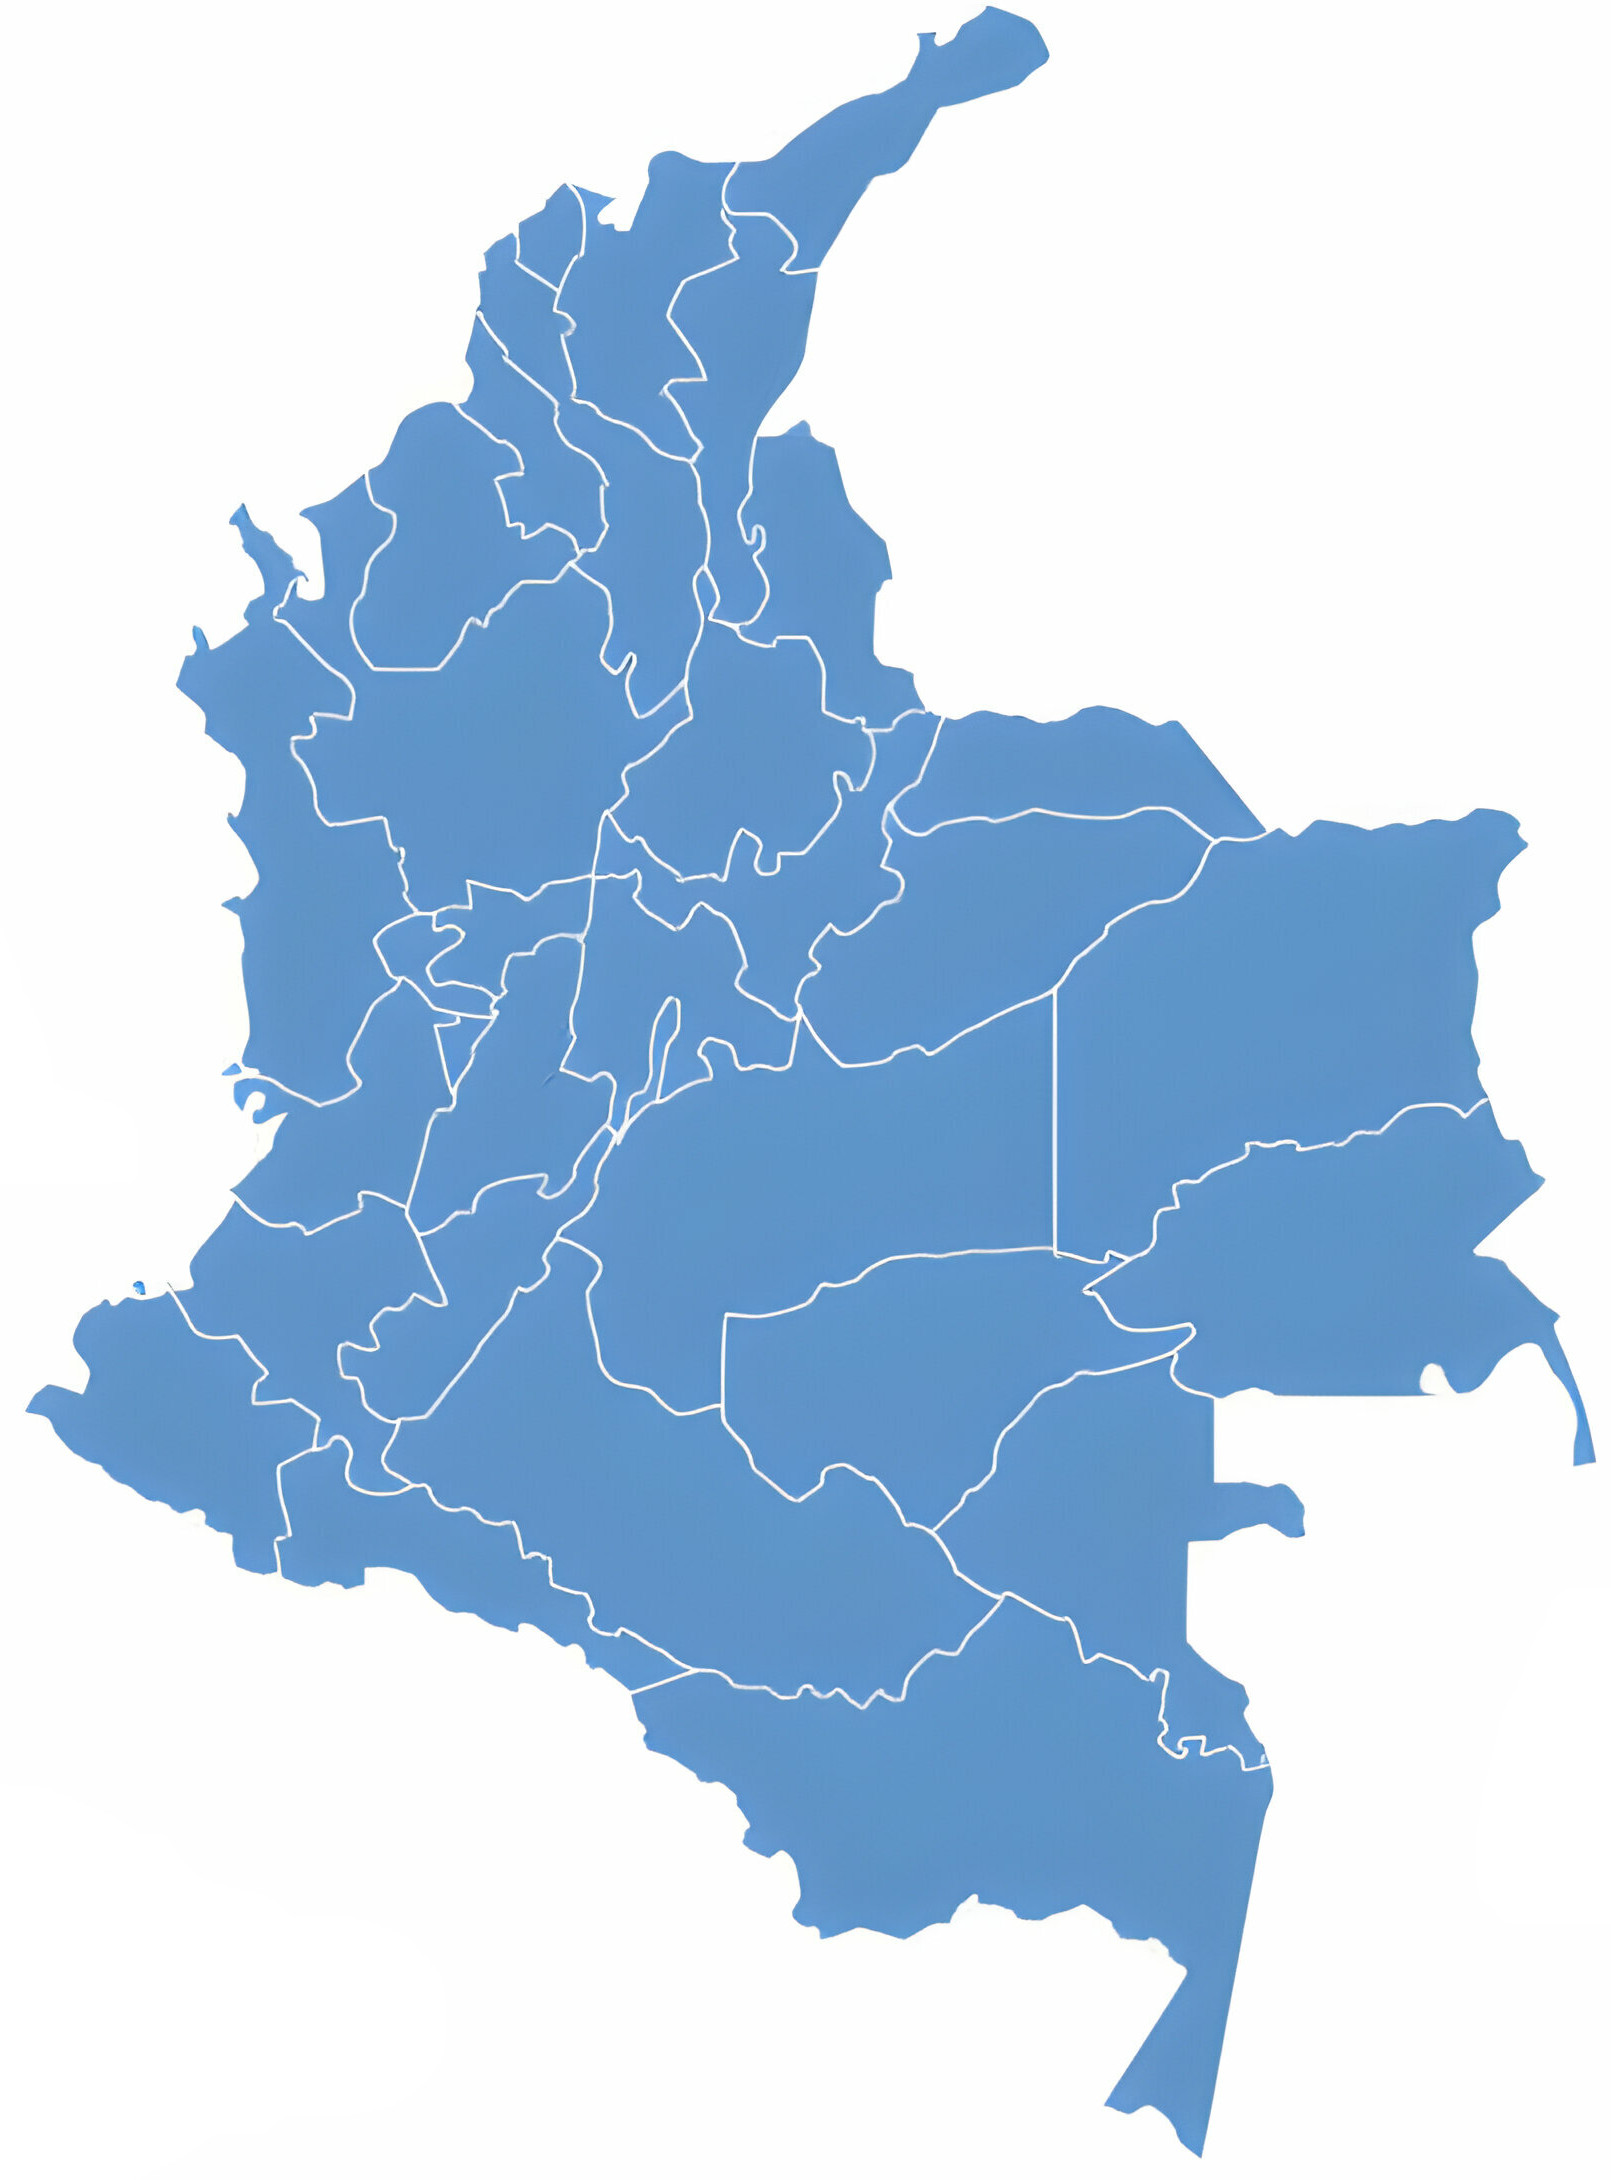
\includegraphics[width=0.5\columnwidth]{images/platanal}
\end{figure}

\end{columns}

\end{frame}
%
\begin{frame}{Motivation}

\framesubtitle{SPRG: Signal Processing and Recognition Group}

Our research group develops \textbf{transdisciplinary data exchange}
since we know that it exposes novel approaches and supports collaborative
discoveries \textbf{across academic areas} \cite{gomezestrategia,aguirre2023feet}.
\begin{columns}[t]

\column[b]{0.5\textwidth}
\begin{itemize}
\item {\scriptsize{}Data heterogeneity.}{\scriptsize\par}
\item {\scriptsize{}Handling unstructured data.}{\scriptsize\par}
\item {\scriptsize{}Real-Time Data Processing and Exchange.}{\scriptsize\par}
\item {\scriptsize{}Privacy and security regulations.}{\scriptsize\par}
\item {\scriptsize{}Interoperability and accessibility.}{\scriptsize\par}
\item {\scriptsize{}Scalability and efficient management.}{\scriptsize\par}
\end{itemize}

\column[b]{0.5\textwidth}

\begin{figure}
\centering{}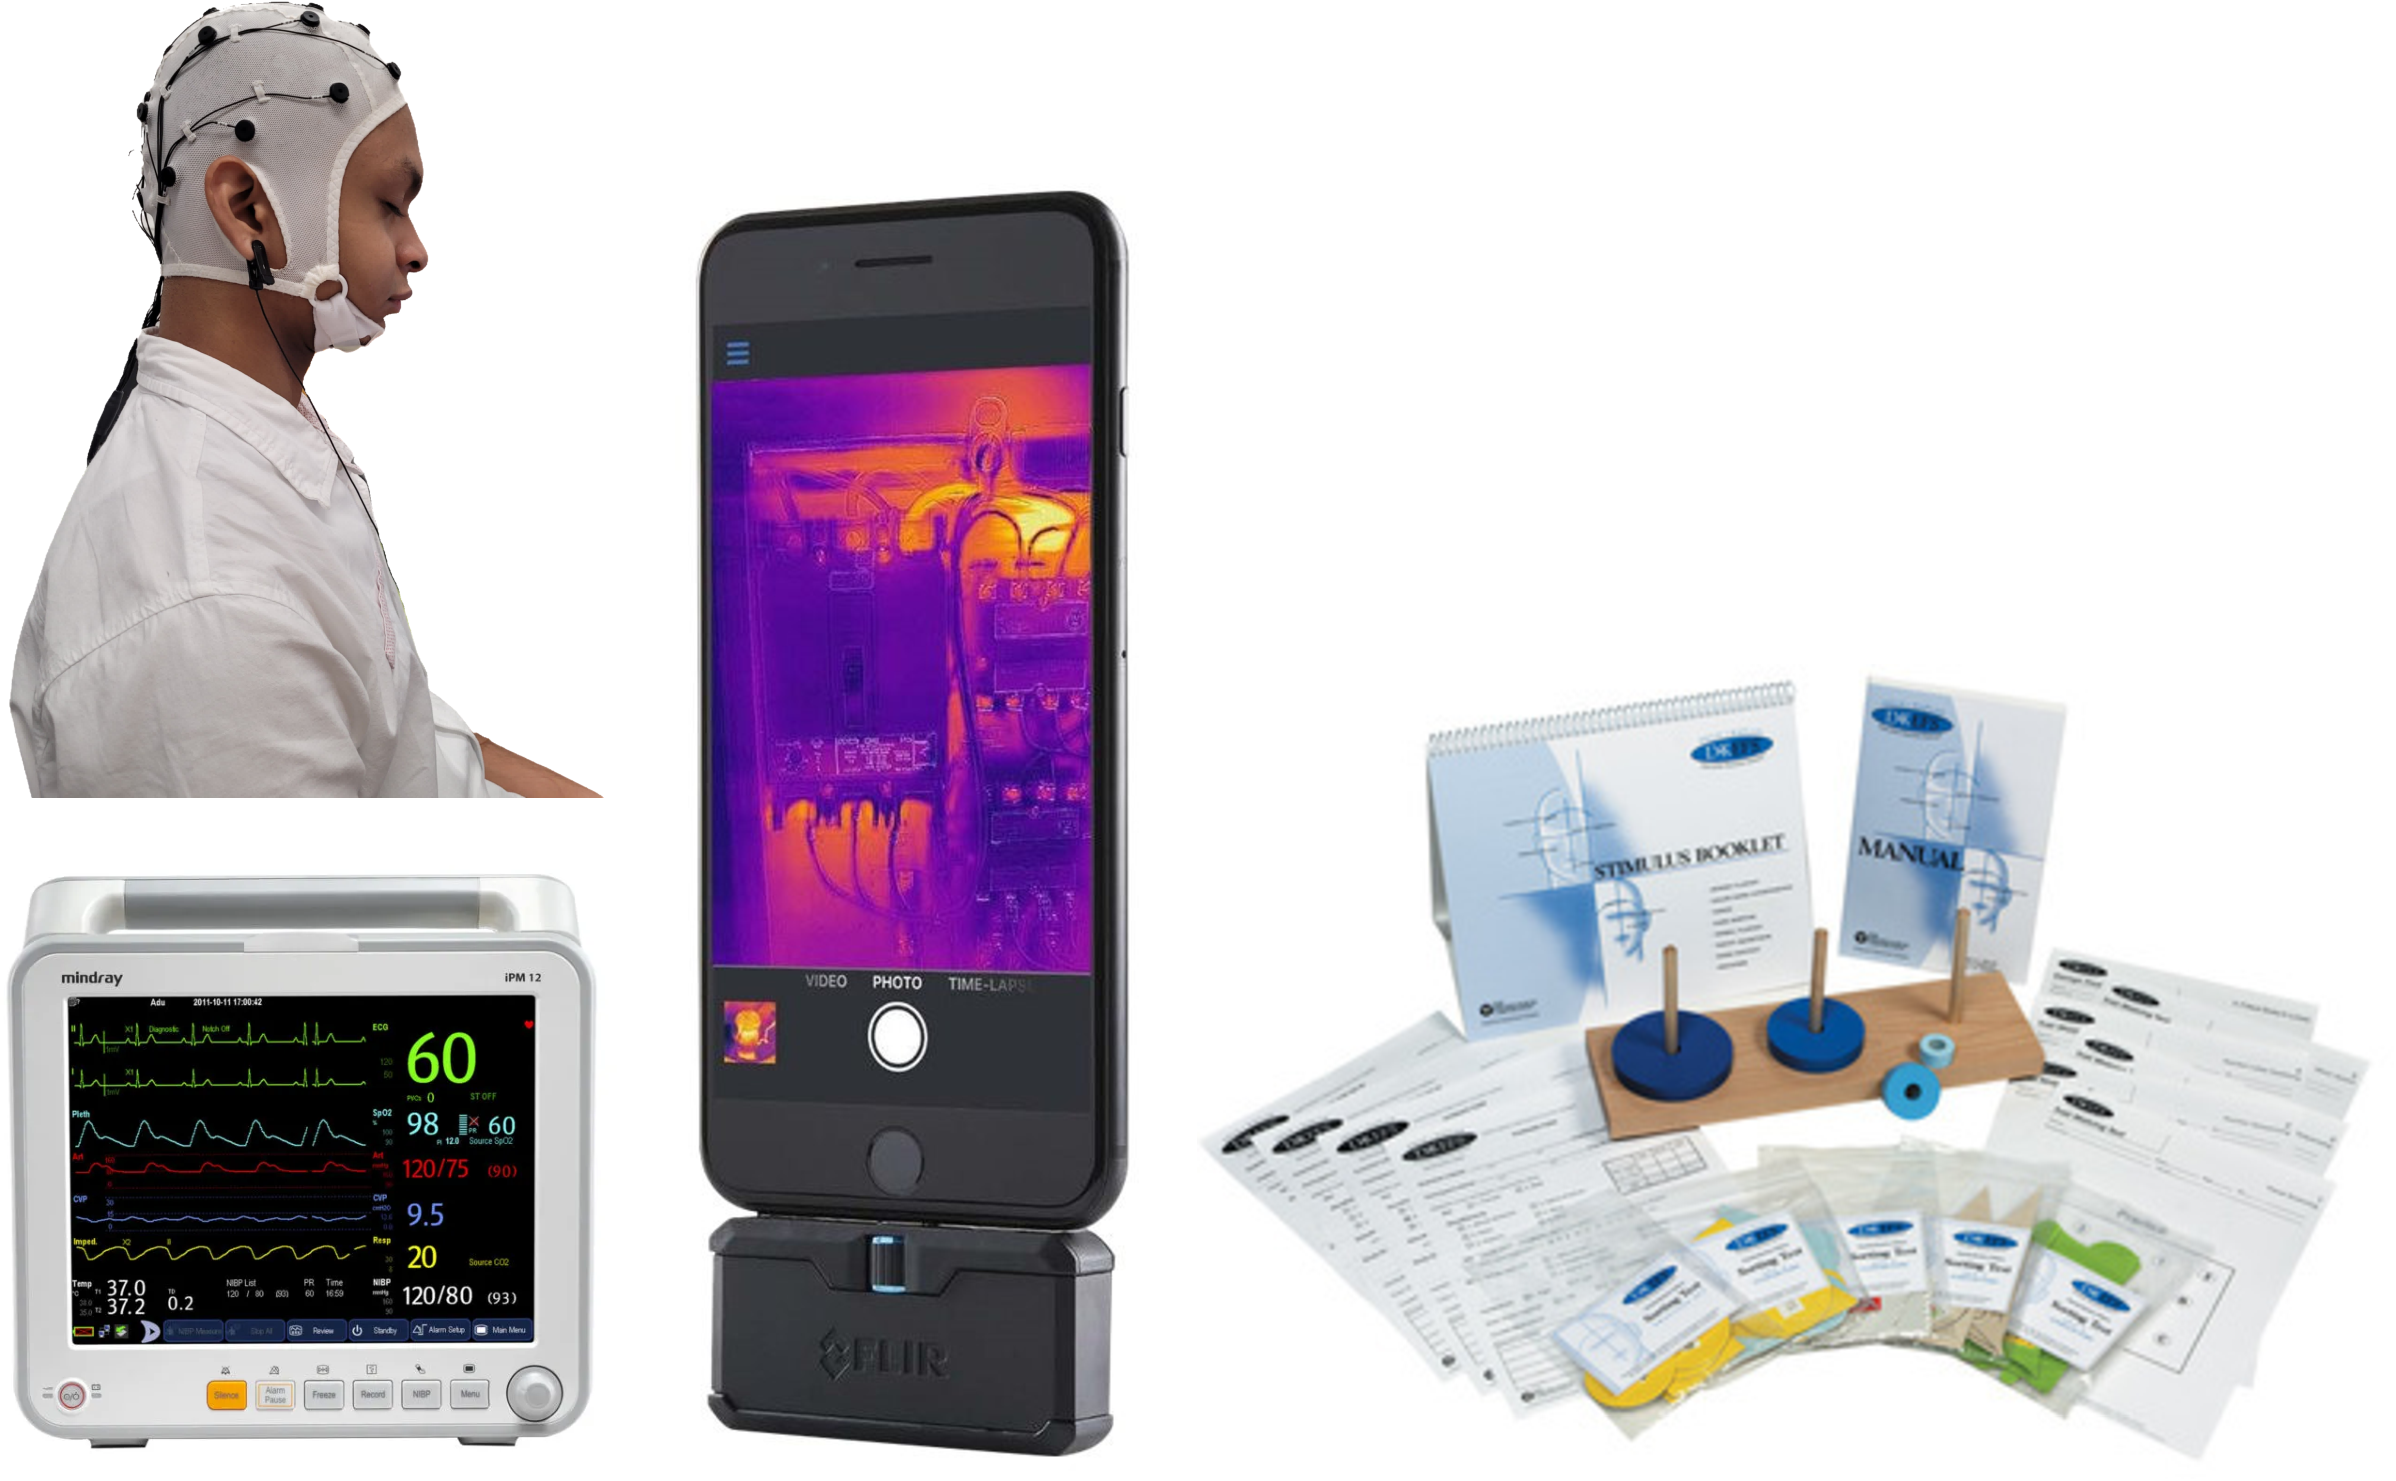
\includegraphics[width=1\columnwidth]{images/research}
\end{figure}

\end{columns}

\end{frame}

\section{Problem statement}
\begin{frame}{Problem statement}

\framesubtitle{Limitations of Data Exchange Methodologies}

 
\begin{columns}[t]

\column{0.5\textwidth}
\begin{description}
\item [{{\scriptsize{}APIs:}}] {\scriptsize{}Request rate, security, and
provider stability/changes limit them \cite{velepucha2023survey}.}{\scriptsize\par}
\end{description}
\vspace{1cm}

\begin{description}
\item [{{\scriptsize{}Messaging:}}] {\scriptsize{}Distributed system scalability,
delivery assurance, state management, and security issues \cite{fang2019integrating}.}{\scriptsize\par}
\end{description}

\column{0.5\textwidth}
\begin{description}
\item [{{\scriptsize{}ETL:}}] {\scriptsize{}Data quality-dependent performance
and complexity concerns with big amounts of different data \cite{abdelhafiz2021sharding}.}{\scriptsize\par}
\end{description}
\vspace{1cm}

\begin{description}
\item [{{\scriptsize{}File\ Transfer:}}] {\scriptsize{}Security, file
size, and bandwidth issues \cite{ordonez2023blockchain,yi2023compound}.}{\scriptsize\par}
\end{description}
\end{columns}

\end{frame}
%
\begin{frame}{Problem statement}

\framesubtitle{API Request Limits}

API request \textbf{rate limits} may cause data transmission difficulties,
especially in multimodal and real-time situations, and make API provider
changes \textbf{harder to adapt} and maintain \cite{Malki2022Impact,Malki2023Combining}.

\begin{figure}
\centering{}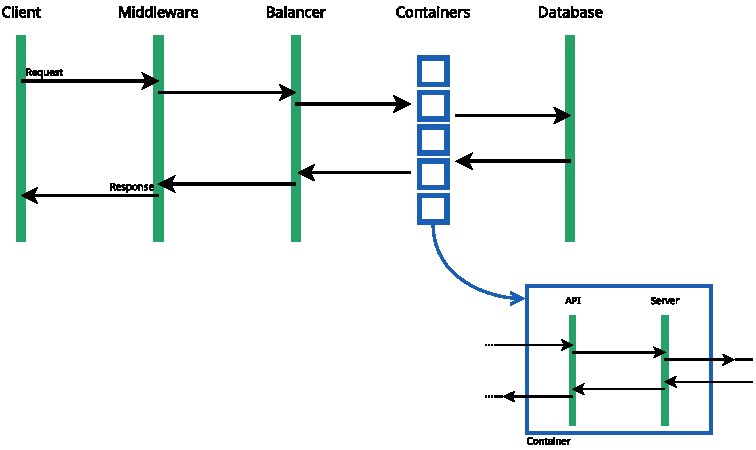
\includegraphics[height=0.35\paperheight]{images/diagrams/API_01}
\end{figure}

\end{frame}
%
\begin{frame}{Problem statement}

\framesubtitle{Messaging Scalability}

Scalability and delivery certainty problems in distributed messaging
systems can lead to the \textbf{loss or delay of messages}, which
can have a severe influence on the \textbf{efficiency and reliability}
of communication in real-time and multimodal contexts \cite{Basin2020Scalable,Arellanes2020Evaluating}.

\begin{figure}
\centering{}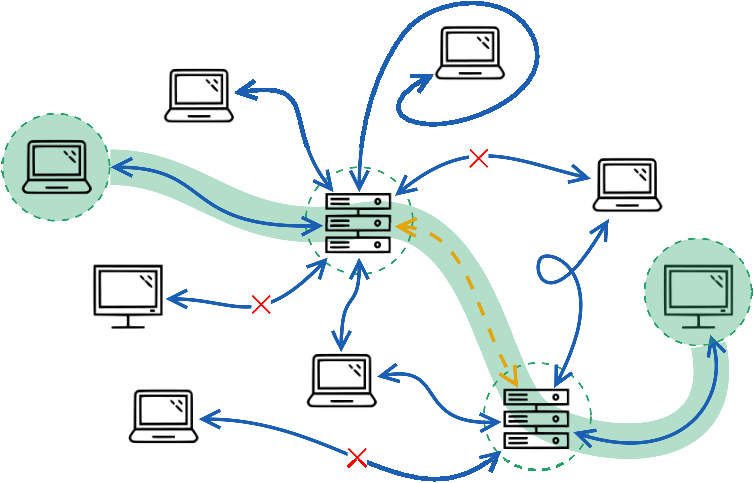
\includegraphics[height=0.35\paperheight]{images/diagrams/MSG_01}
\end{figure}

\end{frame}
%
\begin{frame}{Problem statement}

\framesubtitle{Multimodal ETL \& AI }

Complex multimodal ETL processes can lead to \textbf{inaccurate data
and disruptions} in AI analysis due to challenges with data integration
and real-time data management

\cite{Qaiser2023Comparative,Soussi2021Big-Parallel-ETL:}.

\begin{figure}
\centering{}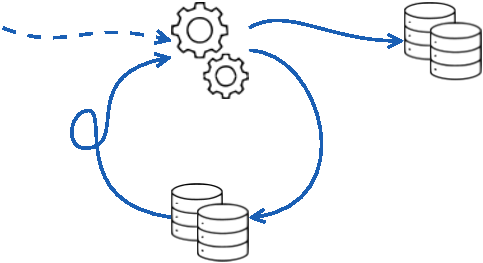
\includegraphics[height=0.35\paperheight]{images/diagrams/ETL_01}
\end{figure}

\end{frame}
%
\begin{frame}{Problem statement}

\framesubtitle{Large-Scale File Transmission}

 

Large-scale file transmission requires efficient and safe administration
of continuous data flow, especially in integrating systems and platforms,
while ensuring data \textbf{integrity} and \textbf{accessibility}
in changing contexts \cite{Zheng2020Design,Yin2023Network}.

\begin{figure}
\centering{}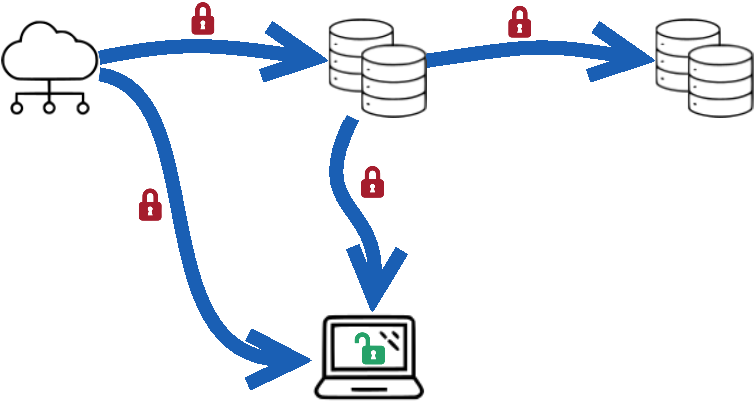
\includegraphics[height=0.35\paperheight]{images/diagrams/FLA_01}
\end{figure}

\end{frame}

\section{State-of-the-Art}
\begin{frame}{State-of-the-Art}

\framesubtitle{APIs Infrastructure Improving}
\begin{itemize}
\item {\footnotesize{}Adaptive REST API Testing with Reinforcement Learning
\cite{kim2023adaptive}.\bigskip{}
}{\footnotesize\par}
\item {\footnotesize{}Dynamic Resources Management Under Limited Communication
Based on Multi-level Agent System\cite{wang2023dynamic}.\bigskip{}
}{\footnotesize\par}
\item {\footnotesize{}Online Task Allocation and Scheduling in Fog IoT using
Virtual Bidding \cite{joshi2022online}.\bigskip{}
}{\footnotesize\par}
\item {\footnotesize{}Event-Triggered Communication Network With Limited-Bandwidth
Constraint for Multi-Agent Reinforcement Learning \cite{hu2021event}.\bigskip{}
}{\footnotesize\par}
\item {\footnotesize{}On the Design and Implementation of Real-Time Resource
Access Protocols \cite{dos2020design}.}{\footnotesize\par}
\end{itemize}
\end{frame}
%
\begin{frame}{Question research}

...
\end{frame}

\section{Aims}
\begin{frame}{General aim}
...

\end{frame}
%
\begin{frame}{Specific aims}

...

\end{frame}

\section{Methodology}
\begin{frame}{Methodology {[}obj1{]}}

...
\end{frame}

\section{Academic advances}
\begin{frame}{Academic advances}

\framesubtitle{Papers, patents and software registers}
\begin{itemize}
\item {[}2023{]} Paper published...
\item {[}2022{]} The systems were submitted to the \textbf{Crearlo no es
suficiente} summons for a \emph{patentability search process} with
the \emph{Universidad Nacional de Colombia sede Manizales} as main
beneficiary with the title \textbf{\textquotedbl MÉTODO Y SISTEMA
PARA LA SINCRONIZACIÓN DE MARCADORES ASOCIADOS A SISTEMAS DE INTERFAZ
CEREBRO-COMPUTADOR\textquotedbl}, postulation \emph{ID 343 }and
Application number \emph{NC2022/0007405} from May 28, 2022.
\item {[}2022{]} A script developed with BCI-Framework for\textbf{ Motor
imagery paradigm with game-based stimulus (Pacman interface)} was
submitted to the software register in the \emph{Universidad Nacional
de Colombia sede Manizales}.
\end{itemize}
\end{frame}

\section{Acknowledgements}
\begin{frame}{Acknowledgements}

...
\end{frame}

\section{References}
\begin{frame}[allowframebreaks]{References}

{\tiny{}\bibliographystyle{apalike}
\bibliography{references}
}{\tiny\par}

\end{frame}

\end{document}
